\documentclass[a4paper,11pt,abstracton,hidelinks]{scrartcl}

\usepackage[margin=3cm]{geometry}
\usepackage{graphicx}
\usepackage[UKenglish]{babel}
\usepackage{csquotes}
\usepackage[style=numeric,citestyle=numeric,backend=biber,sorting=none,doi=false,url=false]{biblatex}
\usepackage{float}
\usepackage[export]{adjustbox}
\usepackage[T1]{fontenc}
\usepackage{lmodern}
\usepackage[textsize=tiny]{todonotes}
\usepackage[labelsep=period,font=small,labelfont=bf,format=plain]{caption}
\captionsetup[table]{
  position=above,
  belowskip=10pt,
  aboveskip=0pt,
}
\usepackage[group-separator={,}]{siunitx}
\usepackage{booktabs}
\usepackage{pdflscape}
\usepackage{tablefootnote}
\usepackage{authblk}
\usepackage{threeparttable}
\usepackage{afterpage}
\usepackage{lineno}
\linenumbers
\usepackage{setspace}
\usepackage{hyperref}
\doublespacing

\newcommand{\beginsupplement}{%
  \setcounter{table}{0}
  \renewcommand{\thetable}{S\arabic{table}}%
  \setcounter{figure}{0}
  \renewcommand{\thefigure}{S\arabic{figure}}%
}


% TODO create refs.bibmicrosoft 
\addbibresource{refs.bib}


\title{
Genome variation and population structure among 1,142 mosquitoes of the African malaria vector species \emph{Anopheles gambiae} and \emph{Anopheles coluzzii}
}



\author[1]{\small The \emph{Anopheles gambiae} 1000 Genomes Consortium}
\affil[1]{\footnotesize A list of consortium members appears at the end of the paper}

\begin{document}

\maketitle


%%%%%%%%%%%%%%%%%%%%%%%%%%%%%%%%%%%%%%%%%%%%%%%%%%%%%%%%%%%%%%%%%%%%%%%%%%%%%%%
%%%%%%%%%%%%%%%%%%%%%%%%%%%%%%%%%%%%%%%%%%%%%%%%%%%%%%%%%%%%%%%%%%%%%%%%%%%%%%%
\begin{abstract}


%%
Mosquito control remains a central pillar of efforts to reduce malaria burden in sub-Saharan Africa.
%
However, insecticide resistance is entrenched in malaria vector populations, and countries with high malaria burden face a daunting challenge to sustain malaria control with a limited set of surveillance and intervention tools. 
%
Here we report on the second phase of a project to build an open resource of high quality data on genome variation among natural populations of the major African malaria vector species \textit{Anopheles gambiae} and \textit{Anopheles coluzzii}. 
%
We analysed whole genomes of 1,142 individual mosquitoes sampled from the wild in 13 African countries, and a further 234 individuals comprising parents and progeny of 11 lab crosses. 
%
The data resource includes high confidence single nucleotide polymorphism (SNP) calls at 57 million variable sites, genome-wide copy number variation calls, and haplotypes phased at biallelic SNPs.
%
We used the SNP data to analyse genetic population structure, compute allele frequencies, and characterise genetic diversity within and between populations.
%
We illustrate the utility of these data by investigating species differences in isolation by distance, genetic variation within proposed gene drive target sequences, and patterns of resistance to pyrethroid insecticides.
%
This data resource provides a foundation for developing new operational systems for molecular surveillance, and for accelerating research and development of new vector control tools.
%%

\end{abstract}


%%%%%%%%%%%%%%%%%%%%%%%%%%%%%%%%%%%%%%%%%%%%%%%%%%%%%%%%%%%%%%%%%%%%%%%%%%%%%%%
%%%%%%%%%%%%%%%%%%%%%%%%%%%%%%%%%%%%%%%%%%%%%%%%%%%%%%%%%%%%%%%%%%%%%%%%%%%%%%%
\section*{Introduction}


%% Need for molecular surveillance. Need for open genomic data resources to underpin surveillance.
%
The 10 countries with the highest malaria burden in Africa account for 65\% of all malaria cases globally, and attempts to reduce that burden are facing significant challenges \cite{WHO2018b}.
%
Not least among these, resistance to pyrethroid insecticides is widespread throughout African malaria mosquito populations, potentially compromising the efficacy of mosquito control interventions which remain at the core of global malaria strategy \cite{Hemingway2016, WHO2018a}.
%
There is a broad consensus that further progress cannot be made if interventions are applied blindly, but must instead be targeted and adapted based on data from epidemiological and entomological surveillance \cite{WHO2015}.
%
Genome sequencing technologies are considered to be a key component of future malaria surveillance systems, providing insights into evolutionary and demographic events in mosquito and parasite populations that are otherwise difficult to obtain \cite{Ishengoma2019}.
%
Genomic surveillance systems will not work in isolation, but will depend on high quality open genomic data resources, including baseline data on genome variation from multiple mosquito species and geographical locations, against which comparisons can be made and inferences regarding new events can be drawn.
%%

%% Need to accelerate malaria vector research and development of new vector control tools. Role of open genomic data in accelerating R&D.
%
Better surveillance can increase the impact and longevity of available mosquito control tools, but sustaining malaria control will also require the development and deployment of new mosquito control tools \cite{WHO2015}.
%
This includes repurposing existing insecticides not previously used in public health \cite{Oxborough2019, Lees2019}, developing entirely new insecticide classes, and developing tools that don't rely on insecticides, such as genetic modification of mosquito populations \cite{kyrou2018}.
%
Research and development of new mosquito control tools has been greatly facilitated by the availability of open genomic data resources, including high quality genome assemblies and annotations \cite{Holt2002, sharakhova2007update}, and more recently by high quality resources on genetic variation among natural mosquito populations \cite{Ag1000G2017}. 
%
Further expansion of these open data resources to incorporate unsampled mosquito populations and new types of genetic variation can provide new insights into a range of biological and ecological processes, and help to accelerate scientific discovery from basic biology through to operational research.
%%


%% Introduction to Ag1000G. Summary of Ag1000G phase 1. Limitations of Ag1000G phase 1.
%
The Anopheles gambiae 1000 Genomes project\footnote{\url{https://www.malariagen.net/projects/ag1000g}} (Ag1000G) was established in 2013 to build a large scale open data resource on natural genetic variation in malaria mosquito populations.
%
The Ag1000G project forms part of the Malaria Epidemiology Network\footnote{\url{https://www.malariagen.net}} (MalariaGEN), a data-sharing community of researchers investigating how genetic variation in humans, mosquitoes and malaria parasites can inform the biology, epidemiology and control of malaria.
%
The first phase of the Ag1000G project released data from whole genome Illumina deep sequencing of mosquitoes from 8 African countries, including SNP calls and phased haplotypes \cite{Ag1000G2017}.
%
Mosquitoes were sampled from a broad geographical range, spanning Guinea-Bissau in West Africa to Kenya in East Africa.
%
Both \textit{Anopheles gambiae} and \textit{Anopheles coluzzii} were sampled, two closely related sibling species within the \textit{Anopheles gambiae} species complex \cite{coetzee2013}.
%
Genetic diversity was found to be high in most populations, but there were marked patterns of population structure, and clear differences between populations in the magnitude and architecture of genetic diversity, indicating complex and varied demographic histories.
%
However, both of these species have a large geographical range \cite{wiebe2017}, and many countries and ecological settings are not represented in the Ag1000G phase 1 resource.
%
Also, only SNPs were studied in Ag1000G phase 1, but other types of genetic variation are known to be important.
%
In particular, copy number variation (CNV) has long been suspected to play a key role in insecticide resistance \cite{schimke1978, devonshire1991, weetman2015}, but no previous attempts to call genome-wide CNVs have been made in these species.
%%


%% Introduction to Ag1000G phase 2.
%
This paper describes the data resource produced by the second phase of the Ag1000G project.
%
Within this phase, sampling and sequencing was expanded to include additional wild-caught mosquitoes collected from five countries not represented in phase 1.
%
This includes three new locations with \textit{Anopheles coluzzii}, providing greater power for genetic comparisons with \textit{Anopheles gambiae}, and two island populations, providing a useful reference point to compare against mainland populations.
%
Seven new lab crosses are also included, providing a substantial resource for studying genome variation and recombination within known pedigrees.
%
In this phase we studied both SNPs and CNVs, and rebuilt a haplotype reference panel using all wild-caught specimens.
%
Here we describe the data resource, and use it to re-evaluate major population divisions and characterise genetic diversity.
%
We also illustrate the broad utility of the data by comparing geographical population structure between the two mosquito species to investigate evidence for differences in dispersal behaviour; analyse genetic diversity within a gene in the sex-determination pathway currently targeted for gene drive development; and provide some preliminary insights into the prevalence of different molecular mechanisms of pyrethroid resistance.
%%


%%%%%%%%%%%%%%%%%%%%%%%%%%%%%%%%%%%%%%%%%%%%%%%%%%%%%%%%%%%%%%%%%%%%%%%%%%%%%%%
%%%%%%%%%%%%%%%%%%%%%%%%%%%%%%%%%%%%%%%%%%%%%%%%%%%%%%%%%%%%%%%%%%%%%%%%%%%%%%%
\section*{Results}


\subsection*{Population sampling and sequencing}


%% Paragraph on population sampling and sequencing.
%
We performed whole genome sequencing of 377 individual wild-caught mosquitoes, including individuals collected from 3 countries (The Gambia, Cote d'Ivoire, Ghana) and two oceanic islands (Bioko, Mayotte) not represented in the previous project phase. 
%
We also sequenced 152 individuals comprising parents and progeny from seven lab crosses, where parents were drawn from the Ghana, Kisumu, Pimperena, Mali and Akron colonies. 
%
We then combined these data with the sequencing data previously generated during phase 1 of the project, to create a total resource of data from 1,142 wild-caught mosquitoes (1,058 female, 84 male) from 13 countries (Figure 1; Table 1) and 234 mosquitoes from 11 lab crosses (Table S1). 
%
As in the previous project phase, all mosquitoes were sequenced individually on Illumina technology using 100 bp paired-end reads to a target depth of 30X, and only mosquitoes obtaining a mean depth above 15X were included in the final resource. 
%%


\begin{figure}[H]
	\begin{center}
		\includegraphics*[width=5.8in]{artwork/collection_site_map.jpg}
	\end{center}
	\caption{Ag1000G phase 2 sampling locations. Colour of circle denotes species and area represents sample size. Map colours represent ecosystem classes, dark green designates forest ecosystems; see Figure 9 in \cite{sayre2013} for a compete colour legend.}
	\label{fig:sample_map}
\end{figure}


%% Table 1 - Population sampling.
%
\afterpage{%
%\clearpage
% N.B., for some reason using \newgeometry causes page number to get dropped from the subsequent page, so disable for now - not needed if using \footnotesize.
\newgeometry{margin=2cm}
\begin{landscape}
\thispagestyle{empty}
\begin{table}[h]
  \footnotesize
  \centering
  \begin{threeparttable}

  \caption{
%
\textbf{Ag1000G phase 2 sampling locations}.
}

  \label{table:sampling_locations}

  
\begin{tabular}{lllcccccc}
\toprule
\multicolumn{6}{c}{\textbf{Collection}} &
\multicolumn{3}{c}{\textbf{\emph{Anopheles} species counts}}\\
\cmidrule(r){1-6}
\cmidrule(r){7-9}
Country & 
Location & 
Site &
Year &
Latitude & 
Longitude & 
\emph{gambiae} & 
\emph{coluzzii} & 
Unknown\\
\midrule

Angola & Luanda &  & 2009 & -8.8210 & 13.2910 & 0 & 78 & 0 \\

Burkina Faso & Bana &  & 2012 & 11.2330 & -4.4720 & 20 & 40 & 0 \\

 & Pala &  & 2012 & 11.1500 & -4.2350 & 46 & 10 & 0 \\

 & Souroukoudinga &  & 2012 & 11.2350 & -4.5350 & 26 & 25 & 0 \\

Cameroon & Daiguene &  & 2009 & 4.7770 & 13.8440 & 96 & 0 & 0 \\

 & Gado Badzere &  & 2009 & 5.7470 & 14.4420 & 73 & 0 & 0 \\

 & Mayos &  & 2009 & 4.3410 & 13.5580 & 105 & 0 & 0 \\

 & Zembe Borongo &  & 2009 & 5.7470 & 14.4420 & 23 & 0 & 0 \\

Cote d'Ivoire & Tiassale &  & 2012 & 5.8984 & -4.8229 & 0 & 71 & 0 \\

Equatorial Guinea & Bioko &  & 2002 & 3.7000 & 8.7000 & 9 & 0 & 0 \\

France & Mayotte & Bouyouni & 2011 & -12.7378 & 45.1417 & 1 & 0 & 0 \\

 &  & Combani & 2011 & -12.7787 & 45.1429 & 5 & 0 & 0 \\

 &  & Karihani Lake & 2011 & -12.7965 & 45.1217 & 3 & 0 & 0 \\

 &  & Mont Benara & 2011 & -12.8570 & 45.1552 & 2 & 0 & 0 \\

 &  & Mtsamboro Forest Reserve & 2011 & -12.7027 & 45.0811 & 1 & 0 & 0 \\

 &  & Mtsanga Charifou & 2011 & -12.9907 & 45.1557 & 8 & 0 & 0 \\

 &  & Sada & 2011 & -12.8521 & 45.1039 & 4 & 0 & 0 \\

Gabon & Libreville &  & 2000 & 0.3840 & 9.4550 & 69 & 0 & 0 \\

Gambia, The & Njabakunda & Kerr Birom Kardo & 2011 & 13.5500 & -15.9000 & 0 & 0 & 19 \\

 &  & Kerr Sama Kuma & 2011 & 13.5500 & -15.9000 & 0 & 0 & 8 \\

 &  & Maria Samba Nyado & 2011 & 13.5500 & -15.9000 & 0 & 0 & 18 \\

 &  & Sare Illo Buya & 2011 & 13.5500 & -15.9000 & 0 & 0 & 20 \\

Ghana & Koforidua &  & 2012 & 6.0945 & -0.2609 & 0 & 1 & 0 \\

 & Madina &  & 2012 & 5.6685 & -0.2193 & 12 & 12 & 0 \\

 & Takoradi &  & 2012 & 4.9122 & -1.7740 & 0 & 20 & 0 \\

 & Twifo Praso &  & 2012 & 5.6086 & -1.5493 & 0 & 22 & 0 \\

Guinea & Koraboh &  & 2012 & 9.2500 & -9.9170 & 22 & 0 & 0 \\

 & Koundara &  & 2012 & 8.5000 & -9.4170 & 18 & 4 & 0 \\

Guinea-Bissau & Antula &  & 2010 & 11.8910 & -15.5820 & 0 & 0 & 58 \\

 & Safim &  & 2010 & 11.9569 & -15.6492 & 0 & 0 & 33 \\

Kenya & Kilifi & Junju & 2012 & -3.8620 & 39.7450 & 0 & 0 & 16 \\

 &  & Mbogolo & 2012 & -3.6350 & 39.8580 & 0 & 0 & 32 \\

Uganda & Tororo & Nagongera & 2012 & 0.7700 & 34.0260 & 112 & 0 & 0 \\

\bottomrule
\end{tabular}



  \end{threeparttable}

\end{table}
\end{landscape}
\restoregeometry
} % end afterpage
%% end Table 1


\subsection*{Genome variation}


%% Paragraph on nucleotide variation, including SNP discovery, genome accessibility and haplotype phasing.
%
Sequence reads from all individuals were aligned to the AgamP4 reference genome \cite{Holt2002, sharakhova2007update} and SNPs were discovered using methods described previously \cite{Ag1000G2017}.
%
In total, we discovered 57,837,885 SNPs passing all variant quality filters. 
%
Of these high quality SNPs, 24\% were found to be multiallelic (three or more alleles), and 11\% were newly discovered in this project phase.
%
We also analysed genome accessibility to identify all genomic positions where read alignments were of sufficient quality and consistency to support accurate discovery and genotyping of nucleotide variation.
%
Similar to the previous project phase, we found that 61\% (140 Mbp) of genome positions were accessible, including 91\% (18 Mbp) of the exome and 58\% (121 Mbp) of non-coding positions.
%
Overall we discovered an average of one variant allele every 1.9 bases of the accessible genome.
%
We then used high quality biallelic SNPs to construct a new haplotype reference panel including all 1,142 wild-caught individuals, via a combination of read-backed phasing and statistical phasing as described previously \cite{Ag1000G2017}. 
%%


%%
In this project phase we also performed a genome-wide CNV analysis, described in detail elsewhere \cite{Lucas2019a}.
%
In brief, for each individual mosquito, we called CNVs by fitting a hidden Markov model to windowed data on depth of sequence read coverage, then compared calls between individuals to identify shared CNVs.
%
The CNV callset comprises 31,335 distinct CNVs, of which 7,086 were found in more than one individual, and 1,557 were present at at least 5\% frequency in one or more populations.
%
CNVs spanned more than 68 Mbp in total and overlapped 7,190 genes.
%
CNVs were significantly enriched in gene families associated with metabolic resistance to insecticides, with three loci in particular (\textit{Cyp6p/aa}, \textit{Cyp9k1}, \textit{Gste}) having a large number of distinct CNV alleles, multiple alleles at high population frequency, and evidence that CNVs are under positive selection.
%
CNVs at these loci are thus likely to be playing an important role in adaptation to mosquito control interventions.
%% 


\subsection*{Species assignment}


%% Paragraph about species ancestry, reporting results of AIM analysis.
%
The conventional molecular assay for differentiating \textit{An. gambiae} from \textit{An. coluzzii} is based on a fixed genetic difference at a single locus on the X chromosome \cite{santolamazza2008}.
%
In the first phase of Ag1000G, we compared the results of this assay with genotypes at 506 ancestry-informative SNPs distributed across all chromosome arms, and found that in some cases the conventional assay was not concordant with species ancestry at other genome locations.
%
In particular, all individuals from two sampling locations (Kenya, Guinea-Bissau) carried a mixture of \textit{An. gambiae} and \textit{An. coluzzii} alleles, creating uncertainty regarding the appropriate species assignment \cite{Ag1000G2017}. 
%
Applying the same analysis to the new samples in Ag1000G phase 2, we found that mosquitoes from The Gambia also carried a mixture of alleles from both species, in similar proportions to mosquitoes from Guinea-Bissau (Figure \ref{fig:aim}).
%
In all other locations, alleles at ancestry-informative SNPs were concordant with conventional diagnostics \cite{scott1993, fanello2002, santolamazza2008}, except on chromosome arm 2L where there has been a known introgression event carrying an insecticide resistance allele from \textit{An. gambiae} into \textit{An. coluzzii} \cite{weill2000, diabate2004, clarkson2014, norris2015}.
%
We observed this introgression in \textit{An. coluzzii} from both Burkina Faso and Angola in the phase 1 cohort, and it was also present among \textit{An. coluzzii} from Cote d'Ivoire, Ghana and Guinea in the phase 2 cohort, confirming that this introgression has spread widely throughout \textit{An. coluzzii} populations.
%%


\begin{figure}[H]
	\begin{center}
		\includegraphics*[width=6.3in]{artwork/main_pca.jpeg}
	\end{center}
	\caption{Principal component analysis of wild-caught mosquitoes using biallelic SNPs from euchromatic regions of Chromosome 3. Bar-chart shows the percentage of variance explained by each component.}
	\label{fig:pca}
\end{figure}


\subsection*{Population structure}


%% Paragraph with results on population structure.
%
We investigated genetic population structure within the cohort of wild-caught mosquitoes by performing two principal components analyses (PCA), the first using biallelic SNPs from euchromatic regions of Chromosome 3 (Figure \ref{fig:pca}), the second using CNVs from the whole genome (Figure \ref{fig:cnv_pca}).
%
To complement the PCAs, we also used the SNP data to compute two measures of genetic differentiation -- average $F_{ST}$ and rates of rare variant sharing -- between all pairs of 16 populations defined by country of origin and species, excluding \textit{An. coluzzii} from Guinea due to small sample size (Figure \ref{fig:fstdbl}).
%
From these analyses, three major groupings of individuals from multiple countries were evident: \textit{An. coluzzii} from West Africa (Burkina Faso, Ghana, Cote d'Ivoire, Guinea); \textit{An. gambiae} from West and Central Africa (Burkina Faso, Ghana, Guinea, Cameroon, Bioko); individuals with uncertain species status from far West Africa (Guinea-Bissau, The Gambia). 
%
Within each of these groupings, samples clustered together in all principal components, and differentiation between countries was weak, consistent with relatively unrestricted gene flow between countries.
%
Each of the remaining PCA clusters comprised samples from a single country and species (\textit{An. coluzzii} from Angola; \textit{An. gambiae} from Uganda; \textit{An. gambiae} from Gabon, \textit{An. gambiae} from Mayotte; individuals with uncertain species status from Kenya), and each of these populations was relatively strongly differentiated from all other populations, consistent with geographical factors limiting gene flow.
%
A comparison of the two \textit{An. gambiae} island populations is interesting because Mayotte was highly differentiated from all other populations, but individuals from Bioko clustered closely with other West African \textit{An. gambiae}, suggesting that Bioko is not isolated from continental populations despite a physical separation of more than 30 km.
%%


\begin{figure}[H]
	\begin{center}
		\includegraphics*[width=6.3in]{artwork/structure_composite.pdf}
	\end{center}
	\caption{Genetic differentiation between populations. \textbf{(a)} Average allele frequency differentiation ($F_{ST}$) between pairs of populations. The bottom left triangle shows average $F_{ST}$ values between each population pair. The top right triangle shows the Z score for each $F_{ST}$ value estimated via a block-jackknife procedure. \textbf{(b)} Allele sharing in doubleton ($f_{2}$) variants. For each population, we identified the set of doubletons with at least one allele originating from an individual in that population. We then computed the fraction of those doubletons shared with each other population including itself. The height of the coloured bars represent the probability of sharing a doubleton allele between or within populations. Heights are normalized row-wise for each population so that the sum of coloured bars in each row equals 1.
}
	\label{fig:fstdbl}
\end{figure}


%% Paragraph on isolation by distance.
%
The new locations sampled in this project phase allow more comparisons to be made between \textit{An. gambiae} and \textit{An. coluzzii}, and there are many open questions regarding their behaviour, ecology and evolutionary history.
%
For example, it would be valuable to know whether there are any differences in dispersal behaviour between the two species \cite{dao2014, north2019}. 
%
Providing a comprehensive answer to this question is beyond the scope of this study, but we performed a preliminary analysis by estimating Wright's neighbourhood size for each species \cite{wright1946}.
%
This statistic is an approximation for the effective number of potential mates for an individual, and can be viewed as a measurement of how genetic differentiation between populations correlates with the geographical distance between them (isolation by distance).
%
We used Rousset's method for estimating neighbourhood size based on a regression of normalised $F_{ST}$ against the logarithm of geographical distance \cite{rousset1997genetic}.
%
To avoid any confounding effect of major ecological discontinuities, we used only populations from West Africa and Central Africa north of the equatorial rainforest.
%
We found that average neighbourhood sizes are significantly lower in \textit{An. coluzzii} (median=85) than in \textit{An. gambiae} (median=261) (Figure \ref{fig:isolation}), indicating stronger isolation by distance among \textit{An. coluzzii} populations and suggesting a lower rate and/or range of dispersal.
%
We caution, however, that we do not have representation of both species at all sampling locations, and further sampling is needed to confirm this result.
%%


\begin{figure}[H]
	\begin{center}
		\includegraphics*[width=6.3in]{artwork/west_africa_multipanel_edit_NOD.pdf}
	\end{center}
	\caption{Comparison of isolation by distance between \textit{An. coluzzii} and \textit{An. gambiae}. \textbf{(a)} Study region and pairwise $F_{ST}$. \textbf{(b)} Regressions of average genome-wide $F_{ST}$ against geographic distance, following Rousset \cite{rousset1997genetic}. Neighbourhood size is estimated as the inverse slope of the regression line. \textbf{(c)} Difference in neighbourhood size estimates by species, with each point representing a 200kb region of the genome. @@TODO exclude Gabon from the \textit{An. gambiae} analysis, and use $F_{ST}$ from Chromosome 3 only rather than whole genome.}
	\label{fig:isolation}
\end{figure}


\subsection*{Genetic diversity}


%% Introduction to genetic diversity metrics.
%
The populations represented in the Ag1000G phase 2 cohort can serve as a reference point for comparisons with populations sampled by other studies at other times and locations. 
%
To facilitate population comparisons, we characterised genetic diversity within each of 16 populations in our cohort defined by country of origin and species by computing a variety of summary statistics using SNP data from the whole genome.
%
These statistics included nucleotide diversity ($\theta_{\pi}$; Figure \ref{fig:diversity}a), Watterson's estimator ($\theta_{W}$; Figure \ref{fig:theta_w}), Tajima's $D$ (Figure \ref{fig:diversity}b) and site frequency spectra (SFS; Figure \ref{fig:sfs}). 
%
We also estimated runs of homozygosity (ROH; Figure \ref{fig:diversity}c) within each individual and runs of identity by descent (IBD; Figure \ref{fig:diversity}d) between individuals, both of which provide additional information about haplotype sharing and patterns of relatedness within populations. 
%%


\begin{figure}[H]
	\begin{center}
		\includegraphics*[width=6.3in]{artwork/diversity_composite.jpeg}
	\end{center}
	\caption{Genetic diversity within populations. \textbf{(a)} Nucleotide diversity ($\theta_{\pi}$) calculated in non-overlapping 20-kb genomic windows. \textbf{(b)} Tajima's $D$ calculated in non-overlapping 20-kb genomic windows. \textbf{(c)} Runs of homozygosity
(ROH) in individual mosquitoes. \textbf{(d)} Runs of identity by descent, measured between samples.}
	\label{fig:diversity}
\end{figure}


%% Summary of main patterns in the diversity data.
%
The two easternmost populations (Kenya, Mayotte) were outliers in all statistics calculated, with lower diversity, a deficit of rare variants relative to neutral expectation, and a higher degree of haplotype sharing within and between individuals.
%
The Kenyan population was represented in Ag1000G phase 1, and we previously described how the patterns of diversity in this population were consistent with a severe and recent population bottleneck \cite{Ag1000G2017}.
%
The similarities between Kenya and Mayotte suggest that the Mayotte population has also experienced a population bottleneck, which would be expected given that Mayotte is an oceanic island 310 km from Madagascar and 500 km from continental Africa, and may have been colonised by \textit{An. gambiae} via a small number of founding events.
%
Although ROH and IBD were elevated in both populations, Mayotte individuals had a larger number of shorter tracts than Kenyan individuals, which may reflect differences in the timing and/or strength of a bottleneck.
%
In contrast, the \textit{An. gambiae} individuals from Bioko Island had very similar patterns of diversity to \textit{An. gambiae} populations from West and Central Africa, supporting other evidence suggesting that this population is not isolated from continental populations.
%
The additional \textit{An. coluzzii} populations (Ghana, Cote d'Ivoire) were similar to the previously sampled Burkina Faso \textit{An. coluzzii} population, and the newly sampled Gambian population with uncertain species status was similar to the previously sampled Guinea-Bissau population, consistent with evidence from PCA that these populations form groupings with shared demographic histories and ongoing gene flow.
%%


\subsection*{Design of Cas9 gene drives}


%%
%
One of the ways the nucleotide variation data in this resource is being used is to inform the development of gene drives, a novel mosquito control technology using engineered selfish genetic elements to cause mosquito population suppression or modification \cite{burt2003, gantz2015, hammond2016, eckhoff2017, kyrou2018}.
%
Promising results have been obtained with a Cas9 homing endonuclease gene drive targeting a locus in the doublesex gene (\textit{dsx}), which is a critical component of the sex determination pathway \cite{kyrou2018}.
%
This locus was chosen in part because it has extremely low genetic diversity both within and between species in the \textit{An. gambiae} complex \cite{Ag1000G2017}.
%
Low diversity is required because any natural variation within the target sequence could inhibit association with the Cas9 guide RNA and cause resistance to the gene drive \cite{unckless2017}.
%
We reviewed nucleotide variation within \textit{dsx} using the expanded cohort of wild-caught samples in the phase 2 cohort, and found no new nucleotide variants within the target sequence used by Kyrou \textit{et. al.}, other than the previously known SNP at \texttt{2R:48,714,641}, which has been shown not to interfere with the gene drive process in lab populations \cite{kyrou2018}.
%
To facilitate the search for other potential gene drive targets in \textit{dsx} and other genes, we computed allele frequencies for all SNPs in all populations and included those data in the resource.
%
We also compiled a table of all potential Cas9 target sites (23 bp regions with a protospacer-adjacent motif) in the genome, ordered by nucleotide diversity.
%
This table includes @@N viable Cas9 targets that overlap a gene coding sequence and that have complete nucleotide conservation within the Ag1000G phase 2 cohort.
%%


%%
The presence of highly conserved sequences within \textit{dsx} also raises interesting questions regarding the molecular biology of sex determination in \textit{An. gambiae}, which is not fully understood \cite{Scali2005, Krzywinska2016}.
%
Insect sex determination depends on sex-specific splicing of \textit{dsx}, with exon 5 being retained in the female transcript and skipped in the male transcript \cite{Gempe2011}.
%
In \textit{Drosophila melanogaster} this differential splicing depends on female-specific regulatory factors which bind to the exon 5 region of the \textit{dsx} pre-mRNA and promote inclusion of exon 5 within the final transcript \cite{Cline1996, Gempe2011}.
%
Any sequences required for the proper binding of this splicing machinery to the pre-mRNA will be subject to strong purifying selection, because inclusion of exon 5 is essential for sexual differentiation in females \cite{Cline1996, kyrou2018}. 
%
\textit{D. melanogaster} female splice enhancing factors bind to a series of six 13 bp sequences (\textit{dsxRE}s) located in the untranslated region of exon 5 \cite{Cline1996}, and putative homologs of these sequences are present in \textit{An. gambiae}, located towards the boundary with intron 6 \cite{Scali2005}.
%
We examined diversity within the putative \textit{An. gambiae} \textit{dsxRE} sequences and found that five out of six are located in tracts of near-complete nucleotide conservation, consistent with purifying selection and an active role in pre-mRNA binding (Figure \ref{fig:dsx}b).
%
However, the region of conservation at the intron 4/exon 5 boundary targeted for gene drive by Kyrou \textit{et. al.} \cite{kyrou2018} is mysterious, because it is distant from any of these known regulatory sequences.
%
This region of conservation in fact extends over a 200 bp region, including ~50 bp of untranslated sequence within exon 5, the entire coding sequence of exon 5, and 50 bp of intron 4 (Figure \ref{fig:dsx}a).
%
The near-complete conservation of both coding and non-coding sites throughout this region, extending well beyond the immediate vicinity of the splice junction, suggests it is also somehow involved in binding of sex-specific splicing factors, and adds further evidence for fundamental differences in the molecular biology of sex determination between \textit{Anopheles} and \textit{Drosophila} \cite{Scali2005, Krzywinska2016}. 
%


\subsection*{Resistance to pyrethroid insecticides}


%%
Malaria control in Africa depends heavily on mass distribution of long-lasting insecticidal bed-nets (LLINs) impregnated with pyrethroid insecticides \cite{Ranson2016, Churcher2016, Bhatt2015}.
%
Entomological surveillance programs regularly test malaria vector populations for pyrethroid resistance using standardised bioassays, and these data have shown that pyrethroid resistance has become widespread in \textit{An. gambiae} \cite{Hemingway2016, WHO2018a}.
%
However, pyrethroid resistance can be conferred by different molecular mechanisms, and it is not known which molecular mechanisms are responsible for resistance in which mosquito populations.
%
The nucleotide variation data in this resource include 67 non-synonymous SNPs within the \textit{Vgsc} gene that encodes the binding target for pyrethroid insecticides, of which two SNPs (\texttt{L995F}, \texttt{L995S}) are known to confer a pyrethroid resistance phenotype, and one SNP (\texttt{N1570Y}) has been shown to substantially increase pyrethroid resistance when present in combination with \texttt{L995F} \cite{jones2012}. 
%
These SNPs can serve as markers of target-site resistance to pyrethroids, but no study has previously identified any genetic markers of metabolic resistance in \textit{An. gambiae}.
%
Metabolic resistance to pyrethroids is mediated at least in part by increased expression of cytochrome P450 (CYP) enzymes \cite{kwiatkowska13, edi2014, ngufor15, vontas2018}, and we found CNV hot-spots at two loci containing CYP genes \cite{Lucas2019a}.
%
One CYP locus is on chromosome arm 2R and overlaps a cluster of 10 genes, including \textit{Cyp6p3} previously shown to metabolise pyrethroids \cite{muller2008}.
%
The second CYP locus occurs on the X chromosome and spans a single gene, \textit{Cyp9k1}, which has also previously be shown to metabolise pyrethroids \cite{vontas2018}.
%
At each of these loci we found at least 15 distinct CNV alleles, several of which were present in over 50\% of individuals in some populations and were associated with signatures of positive selection \cite{Lucas2019a}.
%
The phenotype of these CNVs remains to be confirmed, but given the multiple lines of evidence it seems reasonable to assume that CNVs at these loci can serve as a molecular marker of CYP-mediated metabolic resistance to pyrethroids.
%%


%%
\begin{figure}[H]
	\begin{center}
		\includegraphics*[width=6.3in]{artwork/pyrethroid_resistance_simplified.jpg}
	\end{center}
	\caption{Pyrethroid resistance genotypes. The geographical distribution of four pyrethroid insecticide resistance genotype states for all 1142 phase 2 wild caught mosquitoes are shown by country across Sub-Saharan Africa. The four pie chart colours represent genotype state: purple - these individuals were either homozygous or heterozygous for at least one of the two widespread \textit{kdr} pyrethroid target site mutations \textit{Vgsc-995F/S}; yellow - these individuals carried any genome amplification within either the \textit{Cyp6} or \textit{Cyp9} gene clusters; orange - these individuals carried at least one \textit{kdr} mutation and one \textit{Cyp} cluster amplification; grey - these individuals carried no known pyrethroid resistance genotypes (no \textit{kdr} or \textit{Cyp} amplifications).}
	\label{fig:ir}
\end{figure}
%%


%%
We constructed an overview of the prevalence of these two pyrethroid resistance mechanisms -- target-site resistance and CYP-mediated metabolic resistance -- within the Ag1000G phase 2 cohort by combining the data on nucleotide and copy number variation.
%
The sampling of these populations was conducted at different times in different locations, and the geographical sampling is relatively sparse, so we cannot draw any general conclusions about the current distribution of resistance from our data.
%
However, some patterns were clear.
%
For example, West African populations of both species (Burkina Faso, Guinea, Cote d'Ivoire) all had more than 84\% of individuals carrying both target-site and metabolic resistance markers.
%
Towards Central Africa (Ghana, Cameroon, Gabon, Angola), target-site resistance was nearly fixed in all populations, but metabolic resistance markers were at lower frequencies, and the samples from Bioko Island carried no resistance markers at all.
%
The Bioko samples were collected in 2000, and so the lack of resistance may be related to the fact that sampling predated any major scale-up of vector control interventions.
%
However, the Gabon samples were also collected in 2000, and show that high levels of target-site resistance were present in at least some populations at that time.
%
In the far West (Guinea Bissau, The Gambia), target-site resistance was absent, but metabolic resistance was present, and thus any molecular surveillance that assays only target site resistance at those locations could be missing an important signal.
%
In East Africa, both Kenya and Uganda had high frequencies of target-site resistance, 88\% and 100\% respectively.
%
However, 81\% of Uganda individuals also had metabolic resistance, whereas only 4\% of Kenyans (two individuals) carried metabolic resistance markers.
%
Denser spatio-temporal sampling and sequencing would enable us to build a more complete picture of the prevalence and spread of these different resistance mechanisms, and would be highly relevant to the design of insecticide resistance management plans.
%%



%%%%%%%%%%%%%%%%%%%%%%%%%%%%%%%%%%%%%%%%%%%%%%%%%%%%%%%%%%%%%%%%%%%%%%%%%%%%%%%
%%%%%%%%%%%%%%%%%%%%%%%%%%%%%%%%%%%%%%%%%%%%%%%%%%%%%%%%%%%%%%%%%%%%%%%%%%%%%%%
\section*{Discussion}


\subsection*{Insecticide resistance surveillance}


%%
%
The Ag1000G phase 2 data resource incorporates both nucleotide and copy number variation from the whole genomes of 1,142 mosquitoes collected from 13 countries spanning the African continent.
%
These data provide a battery of new genetic markers that could be used to expand our capabilities for molecular surveillance of insecticide resistance.
%
Insecticide resistance management is a major challenge for malaria vector control, but the availability of new vector control products is opening up new possibilities. 
%
However, new products may be more expensive than products currently in use, so procurement decisions have to be justified, and resources targeted to areas where they will have the greatest impact.
%
For example, next-generation LLINs are now available which combine a pyrethroid insecticide with either a second insecticide or a synergist compound (PBO) that breaks metabolic resistance by inhibiting CYP enzyme activity in the mosquito.
%
However, CYP-mediated metabolic resistance is only one of several possible mechanisms of pyrethroid resistance that may or may not be present in vector populations being targeted.
%
It would therefore be valuable to survey mosquito populations and determine the prevalence of different pyrethroid resistance mechanisms, both before and after any change in vector control strategy.
%
There are currently no genetic assays for surveillance of pyrethroid metabolic resistance in \textit{An. gambiae} or \textit{An. coluzzii}, but our data resource includes CNVs at two CYP loci (\textit{Cyp6p/aa}, \textit{Cyp9k1}) which could serve as molecular markers of CYP-mediated metabolic resistance.
%
Glutathione S-transferase enzymes have also been implicated in metabolic resistance to pyrethroids as well as other insecticide classes \cite{Pavlidi2018, riveron2014b}, and we found CNVs at the \textit{Gste} locus which could serve as molecular markers of this alternative resistance mechanism, which is not inhibited by PBO.  
%
Further work is needed to characterise the resistance phenotype associated with these CNVs, but the allelic heterogeneity, the high population frequencies, and the evidence for positive selection observed in our data, coupled with previous gene expression and functional studies \cite{kwiatkowska13, edi2014, ngufor15, vontas2018}, all support a metabolic role in pyrethroid resistance.
%
%%


%%
To illustrate the potential for improved molecular surveillance of pyrethroid resistance, we combined the data on known SNP markers of target-site resistance and the novel putative CNV makers of CYP-mediated metabolic resistance, and computed the frequencies of these different resistance mechanisms in the populations we sampled (Figure \ref{fig:ir}).
%
There are clear heterogeneities, with some populations at high frequency for both resistance mechanisms, particularly in West Africa.
%
The presence of CYP-mediated pyrethroid resistance in a population suggests that PBO LLINs might provide some benefit over standard LLINs.
%
However, if other resistance mechanisms are also at high frequency, the benefit of the PBO synergist might be diminished.
%
Current WHO guidance states that PBO LLINs are recommended in regions with ``intermediate levels'' of pyrethroid resistance, but not where resistance levels are high \cite{WHO2017}.
%
This guidance is based on modelling of bioassay data and experimental hut trials, and it is not clear why PBO LLINs are predicted to provide diminishing returns at higher resistance levels, although high levels of resistance presumably correlate with the presence of multiple resistance mechanisms, including mechanisms not inhibited by PBO \cite{Churcher2016}.
%
Without molecular data, however, this guidance is hard to evaluate or improve upon.
%%


%%
%
Ideally, molecular data on insecticide resistance mechanisms would be collected as part of routine entomological surveillance, as well as in field trials of new vector control products, alongside data from bioassays and other standard entomological monitoring procedures.
%
There are several options for scaling up surveillance of new genetic markers, including both whole genome sequencing (WGS) and targeted (amplicon) sequencing with several choices of sequencing technology platform, as well as various PCR-based assays.
%
Assays that target specific genetic loci are attractive in the short term, because of the low cost and infrastructure requirements, and data from Ag1000G have been used successfully to design multiplex assays for the Agena Biosciences iPLEX platform \cite{Lucas2019b} and for Illumina amplicon sequencing (manuscript in preparation).
% 
But targeted assays would need to be updated regularly to ensure all current forms of insecticide resistance are covered, and to capture new forms of resistance as they emerge.
%
None of the samples sequenced in this study were collected more recently than 2012, geographical sampling within each country was limited, and many countries are not yet represented in the resource, therefore there remain important gaps to be filled.
%
The next phase of the Ag1000G project will expand the resource to cover 18 countries, and will include \textit{An. arabiensis} in addition to \textit{An. gambiae} and \textit{An. coluzzii}, and so will address some of these gaps.
%
However, to keep pace with vector populations, regular whole genome sequencing of contemporary populations from a broad selection of sentinel sites will be needed.
%
Fortunately mosquitoes are easy to transport, and the costs of whole genome sequencing continue to fall, so it is reasonable to consider a mixed strategy that includes both whole genome sequencing and targeted assays.
%%


\subsection*{Gene flow}


%%
%
These data also cast some new, and in some cases contrasting, light on the question of gene flow between malaria vector populations.
%
The question is of practical interest, because gene flow is enabling the spread of insecticide resistance between species and across large geographical distances \cite{Ag1000G2017, Clarkson2018}, and needs to be quantified and modelled before any new vector control interventions based on the release of genetically modified mosquitoes could be considered \cite{North2018}.
%
It has also recently been shown that a variety of \textit{Anopheline} species engage in long-distance wind-assisted migration, although data are so far limited to a single area within the Sahelian region \cite{Huestis2019}.
%
We found evidence that isolation by distance is greater for \textit{An. coluzzii} than for \textit{An. gambiae}, at least within West Africa, suggesting that the effective rate of migration is lower in \textit{An. coluzzii}. 
%
However, if \textit{An. coluzzii} really has a lower rate and/or range of dispersal than \textit{An. gambiae}, this is clearly not limiting the spread of insecticide resistance adaptations between countries.
%
For example, among the CNV alleles we discovered at the \textit{Cyp6p/aa}, \textit{Cyp9k1} and \textit{Gste} loci, 7/13 alleles found in \textit{An. coluzzii} had spread to more than one country, compared with 8/27 alleles in \textit{An. gambiae} \cite{Lucas2019a}.
%
There is also an interesting contrast between the spread of pyrethroid target-site and metabolic resistance alleles.
%
Our previous analysis of haplotypes carrying target-site resistance alleles in the Ag1000G phase 1 cohort found that resistance haplotypes had spread to countries spanning the equatorial rainforest and the Rift valley, and had moved between \textit{An. gambiae} and \textit{An. coluzzii} \cite{Ag1000G2017, Clarkson2018}.
%
In the most extreme example, one haplotype (F1) had spread to countries as distant as Guinea and Angola.
%
In contrast, although CNV alleles were commonly found in multiple countries, we did not observe any cases of CNV alleles crossing any of these ecological or biological boundaries, apart from a single allele found in both Gabon and Cameroon \textit{An. gambiae} (\textit{Gste} Dup5).
%
There are multiple possible explanations for this difference, including differences in the strength, timing or spatial distribution of selective pressures, or intrinsic factors such as differences in fitness costs in the absence of positive selection.
%
Further work is required to investigate the selective forces and biological constraints affecting the spread of these different modes of adaptation to insecticide use.
%%


%%
The two island populations sampled in this project phase also provide an interesting contrast.
%
The samples from Mayotte are highly differentiated from mainland \textit{An. gambiae}, have no pyrethroid resistance alleles, and also have patterns of reduced genetic diversity consistent with a reduction in population size, supporting strong isolation.
%
The samples from Bioko, on the other hand, are closely related to West African \textit{An. gambiae}, and have comparable levels of genetic diversity, suggesting ongoing gene flow.
%
However, there are no pyrethroid resistance alleles in our Bioko samples, and although they were collected in 2000, target-site resistance alleles were present in mainland populations at that time, and so the rate of contemporary migration between Bioko and mainland populations remains an open question.
%
A recent study of \textit{An. gambiae} populations on the Lake Victoria islands, separated from mainland Uganda by 4-50 km, found evidence for isolation between island and mainland populations, as well as between individual islands \cite{Bergey2019}.
%
However, some selective sweeps at insecticide resistance loci had spread through both mainland and island populations, thus isolation is not complete and some contemporary gene flow occurs.
%
Resolving these gene flow questions and apparent contradictions will require fitting quantitative models of contemporary migration to genomic data.
%
We previously fitted migration models to pairs of populations using site frequency spectra, but the approach provides poor resolution to differentiate recent from ancient migration rates \cite{Ag1000G2017}.
%
In general, methods that leverage information about haplotype sharing within and between populations should provide the greatest resolution to disentangle ancient from recent demographic events, as well as providing independent estimates for both migration rates and population densities.
%
There is promising recent work in this direction \cite{Al-Asadi2019}, but models have so far only been applied to data from human populations, and the haplotype data we have generated should prove useful for further work to evaluate whether the same models can be applied to malaria vector populations, with sufficient accuracy to support real-world planning of new vector control interventions.
%
%%


\subsection*{Conclusions}


%%
Malaria is becoming a stubborn foe, frustrating global efforts towards elimination in both low and high burden settings.
%
But new vector control tools offer hope, as does the renewed focus on improving surveillance systems and using data to tailor interventions.
%
The genomic data resource we have generated provides a platform from which to accelerate these efforts, demonstrating the potential for data integration on a continental scale.
%
Nevertheless, work remains to fill gaps in these data, by expanding geographical coverage, including other malaria vector species, sampling contemporary populations, and integrating genomic data collection with routine entomological surveillance.
%
We hope that the MalariaGEN data-sharing community and framework for international collaboration can continue to serve as a model for coordinated action.  
%%


%%%%%%%%%%%%%%%%%%%%%%%%%%%%%%%%%%%%%%%%%%%%%%%%%%%%%%%%%%%%%%%%%%%%%%%%%%%%%%%
%%%%%%%%%%%%%%%%%%%%%%%%%%%%%%%%%%%%%%%%%%%%%%%%%%%%%%%%%%%%%%%%%%%%%%%%%%%%%%%
\section*{Methods}


%%%%%%%%%%%%%%%%%%%%%%%%%%%%%%%%%%%%%%%%%%%%%%%%%%%%%%%%%%%%%%%%%%%%%%%%%%%%%%%
\subsection*{Population sampling}

%
Ag1000G phase 2 mosquitoes were collected from natural populations at 33 sites from 23
geographical locations in 13 sub-Saharan African countries. 
%
Samples have been grouped into 16 populations based on collection country and species (Figure \ref{fig:sample_map} \& Table \ref{table:sampling_locations}).
%
Throughout, we use species nomenclature following Coetzee \textit{et al}. \cite{coetzee2013};	
%
prior to	 Coetzee	 \textit{et al}., \textit{An. gambiae} was known as \textit{An. gambiae sensu stricto} (S form) and \textit{An. coluzzii} was known as \textit{An. gambiae sensu stricto} (M form).
%
Details of the eighteen collection sites novel to Ag1000G phase 2 (dates, collection and DNA extraction methods) can be found in the Methods section.
%
Information pertaining to the collection of samples released as part of Ag1000G phase 1 can be found in the supplementary methods of Ag1000G Consortium (2017) \cite{Ag1000G2017}.
%
Unless otherwise stated, the DNA extraction method used for the collections described below was Qiagen DNeasy Blood and Tissue Kit (Qiagen Science, MD, USA).
%%


%
\textbf{C\^{o}te d'Ivoire (CIcol)}: Tiassal\'{e} (-4.823, 5.898) is located in the evergreen forest zone of southern C\^{o}te d'Ivoire.
%
The primary agricultural activity is rice cultivation in irrigated fields.
%
High malaria transmission occurs during the rainy seasons, between May and November.
%
Samples were collected as larvae from irrigated rice fields by dipping between May and Septermber 2012.
%
All larvae were reared to adults and females preserved over silica for DNA extraction.
%
Specimens from this site were all \textit{An. coluzzii}, determined by PCR assay \cite{santolamazza2008}
%%

\textbf{Bioko Island - Equatorial Guinea (GQgam)}: Collections were performed during the rainy season in September, 2002 by overnight CDC light traps in Sacriba of Bioko island (8.7, 3.7).
%
Specimens were stored dry on silica gel before DNA extraction.
%
Specimens contributed from this site were \textit{An. gambiae} females, genotype determined by two assays \cite{scott1993, santolamazza2004}.
%
All specimens had the 2L\textsuperscript{+a}/2L\textsuperscript{+a} karyotype as determined by the molecular PCR diagnostics \cite{White2007}. 
%
These mosquitoes represent a population that inhabited Bioko Island before a comprehensive malaria control intervention initiated in February 2004 \cite{Sharp2007}. 
%
After the intervention \textit{An. gambiae} was declining, and more recently almost only \textit{An. coluzzii} can be found \cite{Overgaard2012}.
%%

%
\textbf{Mayotte Island - France (FRgam)}: Samples were collected as larvae during March-April 2011 in temporary pools by dipping, in Bouyouni (-12.738, 45.143), M'Tsamboro Forest Reserve (-12.703, 45.081), Combani (-12.779, 45.143), Mtsanga Charifou (-12.991, 45.156), Karihani Lake forest reserve (-12.797, 45.122), and Sada (-12.852, 45.104) in Mayotte island.
%
Larvae were stored in 80\% ethanol prior to DNA extraction. 
%
All specimens contributed to Ag1000G phase 2 were \textit{An. gambiae} \cite{santolamazza2004} with the standard 2L\textsuperscript{+a}/2L\textsuperscript{+a} or inverted 2L\textsuperscript{a}/2L\textsuperscript{a} karyotype as determined by the molecular PCR diagnostics \cite{White2007}.
%
The samples were identified as males or females by the sequencing read coverage of the X chromosome using LookSeq \cite{Manske2009}.
%%

%
\textbf{The Gambia (GM)}: Indoor resting female mosquitoes were collected by pyrethrum spray catch from four hamlets around Njabakunda (-15.90, 13.55), North Bank Region, The Gambia between August and October 2011.
%
The four hamlets were Maria Samba Nyado, Sare Illo Buya, Kerr Birom Kardo, and Kerr Sama Kuma; all are within 1 km of each other.
%
This is an area of unusually high hybridization rates between \textit{An. gambiae s.s.} and \textit{An. coluzzii} \cite{Caputo2008, Nwakanma2013}.
%
Njabakunda village is approximately 30 km to the west of Farafenni town and 4 km away from the Gambia River.
%
The vegetation is a mix of open savannah woodland and farmland.
%
With apparent high gene-flow in the region, it is problematic to assign species to these samples.
%%

%
\textbf{Ghana (GHcol/GHgam)}: Twifo Praso (5.609, -1.549) a peri-urban community located in semi-deciduous forest in the Central Region of Ghana.
%
It is an extensive agricultural area characterised by small-scale (vegetable growing) and large-scale commercial farms such as oil palm and cocoa plantations.
%
Mosquito samples were collected as larvae from puddles near farms between September and October, 2012.
%
Madina (5.668,	-0.219) is suburb of Accra within a coastal savanna zone of Ghana. 
%
It is an urban community characterised by myriad vegetable-growing areas.
%
The vegetation consists of mainly grassland interspersed with dense short thickets often less than 5 m high with a few trees.
%
Specimens were sampled from puddles near roadsides and farms between October and December 2012.
%
Takoradi (4.912, -1.774) is the capital city of Western Region of Ghana.
%
It is an urban community located in the coastal savanna zone.
%
Mosquito samples were collected from puddles near road construction and farms between August and September 2012.
%
Koforidua (6.094, -0.261) is a capital city of Eastern Region of Ghana and is located in semi-deciduous forest. 
%
It is an urban community characterized by numerous small-scale vegetable farms. 
%
Samples were collected from puddles near road construction and farms between August and September 2012.
%
Larvae from all collection sites were reared to adults and females preserved over silica for DNA extraction.
%
Both \textit{An. gambiae} and \textit{An. coluzzii} were collected from these sites, determined by PCR assay \cite{santolamazza2008}.
%%

%
\textbf{Guinea-Bissau (GW)}: Mosquitoes were collected in October 2010 using indoor CDC light traps, in the village of Safim (11.957, -15.649), ca. 11 km north of Bissau city, the capital of the country.
%
Malaria is hyperendemic in the region and transmitted by members of the Anopheles gambiae complex (Vicente et al., 2017).
%
\textit{Anopheles arabiensis, An. melas, An. coluzzii} and \textit{An. gambiae}, as well as hybrids between the latter two species, are known to occur in the region \cite{Gordicho2014, Vicente2017}.
%
Mosquitoes were preserved individually on 0.5ml micro-tubes filled with silica gel and cotton. DNA extraction was performed by a phenol-chloroform protocol \cite{Donnelly1999}.
%
Guinea-Bissau is another region where defining species is problematic (Vicente), so no species has been assigned here.
%%


%%%%%%%%%%%%%%%%%%%%%%%%%%%%%%%%%%%%%%%%%%%%%%%%%%%%%%%%%%%%%%%%%%%%%%%%%%%%%%%
\subsection*{Lab crosses}

%%
The Ag1000G phase 2 data release includes the genomes of seven additional lab colony crosses, both parents and offspring (Table \ref{table:colony_crosses}):
%
cross 18-5 (Ghana mother x Kisumu/G3 father, 20 offspring); 37-3 (Kisumu x Pimperena, 20 offspring); 45-1 (Mali x Kisumu, 20 offspring); 47-6 (Mali x Kisumu, 20 offspring); 73-2 (Akron x Ghana, 19 offspring); 78-2 (Mali x Kisumu/Ghana, 19 offspring); 80-2 (Kisumu x Akron, 20 offspring).
%
Father colonies with two names, \textit{e.g.} "Kisumu/G3", signify that the father is from one of these two colonies, but exactly which one is unknown.
%
The	colony labels, \textit{e.g.}	"18-5", are	identifiers used for	
each of the crosses	within the project and	have no special meaning.	
%
Information pertaining to the crosses released as part of Ag1000G phase 1 can be found in the supplementary methods of Ag1000G Consortium (2017) alongside methods for cross creation and processing. \cite{Ag1000G2017}.
%%


%%%%%%%%%%%%%%%%%%%%%%%%%%%%%%%%%%%%%%%%%%%%%%%%%%%%%%%%%%%%%%%%%%%%%%%%%%%%%%%
\subsection*{Whole genome sequencing}

%
Sequencing was performed on the Illumina HiSeq 2000 platform at the Wellcome Sanger Institute.
%
Paired-end multiplex libraries were prepared using the manufacturer's protocol, with the exception that genomic DNA was fragmented using Covaris Adaptive Focused Acoustics rather than nebulization.
%
Multiplexes comprised 12 tagged individual mosquitoes and three lanes of sequencing were generated for each multiplex to even out variations in yield between sequencing runs.
%
Cluster generation and sequencing were undertaken per the manufacturer's protocol for paired-end 100 bp sequence reads with insert size in the range 100-200 bp.
%
Target coverage was 30X per individual.
%%


%%%%%%%%%%%%%%%%%%%%%%%%%%%%%%%%%%%%%%%%%%%%%%%%%%%%%%%%%%%%%%%%%%%%%%%%%%%%%%%
\subsection*{Genome accessibility}

%
For various population-genomic analyses, it is necessary to have a map of which positions in the reference genome can be considered accessible (in which we can confidently call genetic variation).
%
For phase 2 we repeated the phase 1 acccessibility analyses \cite{Ag1000G2017} with 1142 samples and the additional Mendelian error information provided by the 11 crosses (in phase 1 there were four crosses).
%
Following these analyses it was apparent that the phase 1 accessibility classifications were also appropriate in application to phase 2.
%
Reference genome positions were accessible if: 
Not repeat masked by DUST; 
No Coverage <= 0.1\% (at most 1 individual had zero coverage); 
Ambiguous Alignment <= 0.1\% (at most 1 individual had ambiguous alignments); 
High Coverage <= 2\% (20 individuals); 
Low Coverage <= 10\% (114 individuals); 
Low Mapping Quality <= 10\% (114 individuals).
%%


%%%%%%%%%%%%%%%%%%%%%%%%%%%%%%%%%%%%%%%%%%%%%%%%%%%%%%%%%%%%%%%%%%%%%%%%%%%%%%%
\subsection*{Sequence analysis and variant calling}


%%
Sequencing pipelines were unchanged from phase 1 of the Anopheles 1000 genomes project\cite{Ag1000G2017}.
%
Briefly, sequence reads were aligned to the AgamP3 reference genome \cite{sharakhova2007update} using \texttt{bwa v0.6.2}, duplicate reads marked \cite{li2009} and SNPs discovered using \texttt{GATK Unified Genotyper 2.7.4} \cite{van2013} following best practice recommendations. 
%%


%%%%%%%%%%%%%%%%%%%%%%%%%%%%%%%%%%%%%%%%%%%%%%%%%%%%%%%%%%%%%%%%%%%%%%%%%%%%%%%
\subsection*{Reference divergence}

%%
The genomes of \textit{An. coluzzii} and \textit{An. gambiae} samples were similarly diverged from the reference genome used for alignment, AgamP4 \cite{Holt2002}, indicating that unbiased comparisons can be made between the two species based on our results (Fig. \ref{fig:refdiff}a).
%
The similarity in levels of divergence reflect the mixed ancestry of the PEST strain from which the reference genome was derived \cite{Holt2002}.
%
An exception to this is the pericentromeric region of the X chromosome, a known region of divergence between the two species \cite{Ag1000G2017} where the reference genome is closer to \textit{An. coluzzii} than to \textit{An. gambiae}.
%
The similarity of this region to \textit{An. coluzzii} may be due to artificial selection for the X-linked pink eye mutation in the reference strain \cite{Holt2002}, as this originated in the \textit{An. coluzzii} parent it may have led to the removal of any \textit{An. gambiae} ancestry in this region.
%
Reductions in divergence from the reference genome in regions of low recombination are apparent in the centromeres and telomeres, as well as in the large 2La polymorphic inversion in both species \cite{coluzzi2002} (Figure \ref{fig:refdiff}b \& c). 
%%




%%%%%%%%%%%%%%%%%%%%%%%%%%%%%%%%%%%%%%%%%%%%%%%%%%%%%%%%%%%%%%%%%%%%%%%%%%%%%%%
\subsection*{Variant Filtering}


%%
Following Ag1000G phase 1 \cite{Ag1000G2017}, we applied the following SNP filters to reduce the number of false SNP discoveries.
%
We filtered any SNP that occurred at a genome position classified as inaccessible as described in the section on genome accessibility above, thus removing SNPs with evidence for excessively high or low coverage or ambiguous alignment. 
%
We then applied additional filters using variant annotations produced by GATK based on an analysis of Mendelian error in all 11 crosses present in phase 2 and Ti/Tv ratio similar to that described above for the genome accessibility analysis.
%
We filtered any SNP that failed any of the following criteria: QD <5; FS >100; ReadPosRankSum <-8; BaseQRankSum <-50. 
%%


%%
Of 105,486,698 SNPs reported in the raw callset, 57,837,885 passed all quality filters, 13,760,984 (23.8\%) of which were multi-allelic (>= 3 alleles).
%
To produce an analysis-ready VCF file for each chromosome arm, we first removed all non-SNP variants. 
%
We then removed genotype calls for individuals excluded by the sample QC analysis described above, then removed any variants that were no longer variant after excluding individuals. 
%
We then added INFO annotations with genome accessibility metrics and added FILTER annotations per the criteria defined above. 
%
Finally, we added INFO annotations with information about functional consequences of mutations using SNPEFF version 4.1b \cite{Cingolani2012}.
%%


%%%%%%%%%%%%%%%%%%%%%%%%%%%%%%%%%%%%%%%%%%%%%%%%%%%%%%%%%%%%%%%%%%%%%%%%%%%%%%%
\subsection*{Sample quality control}
%
A total of 1285 individual mosquitoes were sequenced as part of Ag1000G phase 2 and included in the cohort for variant discovery. 
%
After variant discovery, quality-control (QC) steps using coverage and contamination filters alongside principal component analysis and meta data concordance were performed to exclude individuals with poor quality sequence and/or genotype data as detailed in \cite{Ag1000G2017}.
%
A total of 143 individuals were excluded at this stage, retaining 1142 individuals for downstream analyses.
%%


%%%%%%%%%%%%%%%%%%%%%%%%%%%%%%%%%%%%%%%%%%%%%%%%%%%%%%%%%%%%%%%%%%%%%%%%%%%%%%%
\subsection*{SNP validation}

We used 11 laboratory crosses, each with between 14-20 progeny, to estimate the error associated with genotyping from short reads. 
%
We defined errors at sites where given confident parental genotypes and Mendelian inheritance, the expected genotypes of progeny are known. 
%
At loci where both parents are homozygous for the reference or alternate allele, we expect the progeny to be homozygous for the reference or alternate allele accordingly.
%
When one parent is homozygous for the reference allele, and the other the alternate allele we expect all progeny to be heterozygous. 
%
Therefore we can generate ascertainment error estimates for heterozygous, homozygous reference and homozygous alternate genotypes.
%
To meet the confidence threshold for homozygous calls, both parents must have 30x coverage, and have no discordant reads.
%
Sites are considered erroneously called if at least 10 progeny have genotypes called at that locus, and one or more do not match the expected genotype. 
%
Sites are considered correctly called if at least 10 progeny have genotypes called and all match the expected genotype. 
%
Error in ascertainment rates are computed over each cross, and errors are reported as the median over all 11 crosses. 
%
%
Raw error rates were 0.72\% (0.39, 2.44) for heterozygotes, 0.07\% (0.03, 0.25) for homozygous reference calls, and 0.82\% (0.37, 1.47) for homozygous alternate calls. 
%
Following variant filtering via QC thresholds and the accessibility map these values dropped to 0.26\% (0.15, 1.23) for heterozygotes, 0.02\% (0.01, 0.12) for homozygous reference calls, and 0.80\% (0.31, 1.51) for homozygous alternate calls. 
%%


%%%%%%%%%%%%%%%%%%%%%%%%%%%%%%%%%%%%%%%%%%%%%%%%%%%%%%%%%%%%%%%%%%%%%%%%%%%%%%%
\subsection*{Haplotype estimation}

%
Haplotype estimation, also known as phasing, was performed on all phase 2 wild-caught individuals using unchanged methodology from phase 1 of the Anopheles 1000 genomes project\cite{Ag1000G2017}.
%
In short, SHAPEIT2 was used to perform statistical phasing with information from sequence reads.
%
Phasing performance was then evaluated by comparison with haplotypes generated from the laboratory crosses and from male X chromosome haplotypes.
%%


%%%%%%%%%%%%%%%%%%%%%%%%%%%%%%%%%%%%%%%%%%%%%%%%%%%%%%%%%%%%%%%%%%%%%%%%%%%%%%%
\subsection*{Population structure}

%
Population structure analyses, AIM, $F_{ST}$ and nucleotide variation PCA were conducted following methods defined in \cite{Ag1000G2017}.
%
All analyses of geographical population structure using SNP data were conducted on euchromatic regions of Chromosome 3, which avoids regions of polymorphic inversions, reduced recombination and unequal divergence from the reference genome \cite{Ag1000G2017}.
%
Unscaled CNV variation PCAs were built from the CNV presence/absence calls \cite{Lucas2019a}, using the "prcomp" function in R \cite{R}.
%
Doubleton sharing was also conducted following \cite{Ag1000G2017}, except that due low sample sizes in GHgam (12 samples), GNcol (4) and GQgam (9) were excluded.  
%%


%%%%%%%%%%%%%%%%%%%%%%%%%%%%%%%%%%%%%%%%%%%%%%%%%%%%%%%%%%%%%%%%%%%%%%%%%%%%%%%
\subsection*{Genetic diversity}

%
Investigations into and utilising genetic diversity, nucleotide diversity, Tajima's D, ROH and IBD (identity by descent), were conducted following methods defined in \cite{Ag1000G2017} but using the phase 2 data release of 1,142 samples.
%
In short, scikit-allel ('1.2.0') was used to calculate windowed averages of nucleotide diversity and Tajima's D \cite{miles2018}, IBDseq version r1206 \cite{browning2015} was used to calculate IBD and an	HMM	implemented	in	Python (available in scikit-allel) was used to calculate ROH.

%%%%%%%%%%%%%%%%%%%%%%%%%%%%%%%%%%%%%%%%%%%%%%%%%%%%%%%%%%%%%%%%%%%%%%%%%%%%%%%
\section*{The \textit{Anopheles gambiae} 1000 Genomes Consortium}

%
\textbf{Data analysis group}: Chris S. Clarkson (phase 2 data lead), Alistair Miles, Nicholas J. Harding, Eric R. Lucas, C. J. Battey, Andrew D. Kern, Michael C. Fontaine, Martin J. Donnelly, Mara K. N. Lawniczak and Dominic P. Kwiatkowski (chair).
%%

%
\textbf{Partner working group}: Martin J. Donnelly (chair), Diego Ayala, Nora J. Besansky, Austin Burt, Beniamino Caputo, Alessandra della Torre, Michael C. Fontaine, H. Charles J. Godfray, Matthew W. Hahn, Andrew D. Kern, Dominic P. Kwiatkowski, Mara K. N. Lawniczak, Janet Midega, Daniel E. Neafsey, Samantha O'Loughlin, Jo\~{a}o Pinto, Michelle M. Riehle, Igor Sharakhov, Daniel R. Schrider, Kenneth D. Vernick, David Weetman, Craig S. Wilding and Bradley J. White.
%%

%
\textbf{Population sampling}: Angola: Arlete D. Troco, Jo\~{a}o Pinto; Bioko: Jorge Cano; Burkina Faso: Abdoulaye Diabat\'{e}, Samantha O'Loughlin, Austin Burt; Cameroon: Carlo Costantini, Kyanne R. Rohatgi, Nora J. Besansky; Cote d'Ivoire: @@TODO; Gabon: Nohal Elissa, Jo\~{a}o Pinto; The Gambia: Davis C. Nwakanma, Musa Jawara; Ghana: @@TODO; Guinea: Boubacar Coulibaly, Michelle M. Riehle, Kenneth D. Vernick; Guinea-Bissau: Jo\~{a}o Pinto, Jo\~{a}o Dinis; Kenya: Janet Midega, Charles Mbogo, Philip Bejon; Mayotte: Gilbert Le Goff, Vincent Robert; Uganda: Craig S. Wilding, David Weetman, Henry D. Mawejje, Martin J. Donnelly; Crosses: David Weetman, Craig S. Wilding, Martin J. Donnelly.
%%

%
\textbf{Sequencing and data production}: Jim Stalker, Kirk Rockett, Eleanor Drury, Daniel Mead, Anna Jeffreys, Christina Hubbart, Kate Rowlands, Alison T. Isaacs, Dushyanth Jyothi, Cinzia Malangone and Maryam Kamali.
%%

%
\textbf{Project coordination}: Victoria Cornelius, Christa Henrichs and Dominic P. Kwiatkowski.


%%%%%%%%%%%%%%%%%%%%%%%%%%%%%%%%%%%%%%%%%%%%%%%%%%%%%%%%%%%%%%%%%%%%%%%%%%%%%%%
%%%%%%%%%%%%%%%%%%%%%%%%%%%%%%%%%%%%%%%%%%%%%%%%%%%%%%%%%%%%%%%%%%%%%%%%%%%%%%%
\beginsupplement


%%%%%%%%%%%%%%%%%%%%%%%%%%%%%%%%%%%%%%%%%%%%%%%%%%%%%%%%%%%%%%%%%%%%%%%%%%%%%%%
\clearpage

\section*{Supplementary figures and tables}

\begin{figure}[H]
	\begin{center}
		\includegraphics*[width=6.3in]{artwork/AIM_figure_scaled.jpg}
	\end{center}
	\caption{Ancestry informative markers (AIM). Rows represent individual mosquitoes (grouped by population) and columns represent SNPs (grouped by chromosome arm). Colours represent species genotype. The column at the far left shows the species assignment according to the conventional molecular test based on a single marker on the X chromosome, which was performed for all populations except Guinea Bissau (GW), The Gambia (GM) and Kenya (KE). The column at the far right shows the genotype for kdr variants in \textit{Vgsc} codon 995. Lines at the lower edge show the physical locations of the AIM SNPs.}
	\label{fig:aim}
\end{figure}


%%%%%%%%%%%%%%%%%%%%%%%%%%%%%%%%%%%%%%%%%%%%%%%%%%%%%%%%%%%%%%%%%%%%%%%%%%%%%%%
\clearpage

\begin{figure}[H]
	\begin{center}
		\includegraphics*[width=6.3in]{notebooks/190-CNV-PCAs/PCA_nonsingle_full.png}
	\end{center}
	\caption{Principal component analysis (components 1-8) of the 1142 wild-caught mosquitoes estimated using copy number variant diversity. Bar-chart shows the percentage of variance explained by each component}
	\label{fig:cnv_pca}
\end{figure}


%%%%%%%%%%%%%%%%%%%%%%%%%%%%%%%%%%%%%%%%%%%%%%%%%%%%%%%%%%%%%%%%%%%%%%%%%%%%%%%
\clearpage

\begin{figure}[H]
	\begin{center}
		\includegraphics*[width=6.3in]{artwork/Watterson_theta.jpeg}
	\end{center}
	\caption{Watterson's theta ($\theta_{W}$) calculated in non-overlapping 20-kb genomic windows.}
	\label{fig:theta_w}
\end{figure}


%%%%%%%%%%%%%%%%%%%%%%%%%%%%%%%%%%%%%%%%%%%%%%%%%%%%%%%%%%%%%%%%%%%%%%%%%%%%%%%
\clearpage

\begin{figure}[H]
	\begin{center}
		\includegraphics*[width=6.3in]{artwork/sfs_supplementary_large.jpg}
	\end{center}
	\caption{SNP density. Plots depict the distribution of allele frequencies (site frequency spectrum) for each population, scaled such that a population with constant size over time is expected to have a constant SNP density over all allele frequencies.}
	\label{fig:sfs}
\end{figure}


%%%%%%%%%%%%%%%%%%%%%%%%%%%%%%%%%%%%%%%%%%%%%%%%%%%%%%%%%%%%%%%%%%%%%%%%%%%%%%%
\clearpage

\begin{figure}[H]
    \textbf{a}
	\begin{center}
        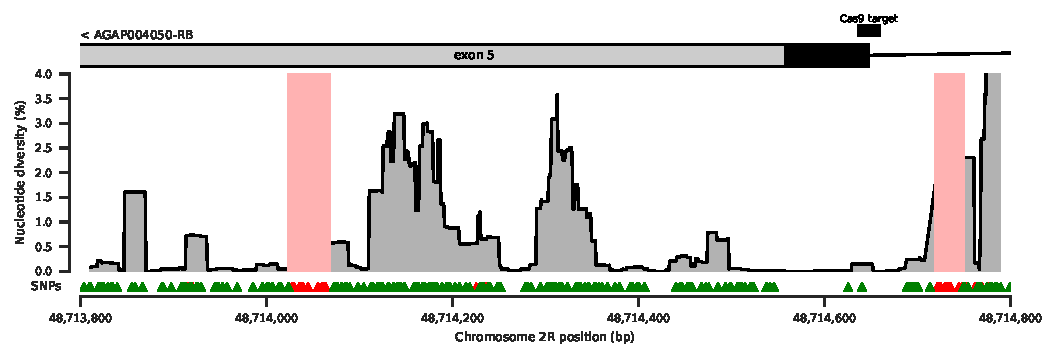
\includegraphics[width=1.0\linewidth]{artwork/dsx_a.pdf}
	\end{center}
    \textbf{b}
	\begin{center}
        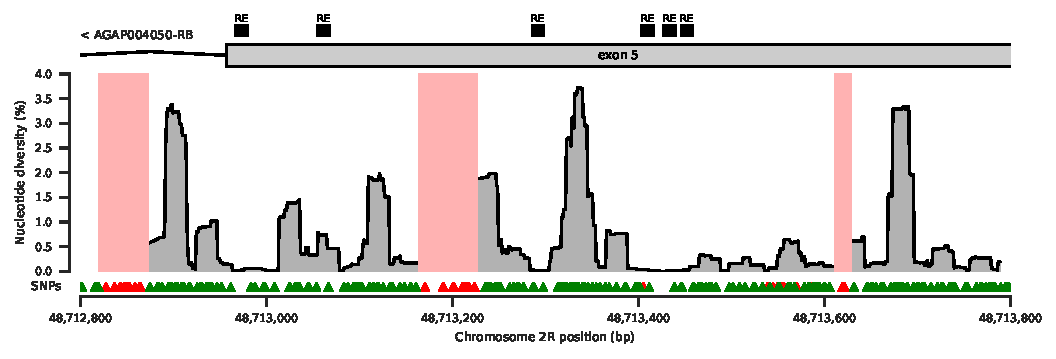
\includegraphics[width=1.0\linewidth]{artwork/dsx_b.pdf}
	\end{center}
    \caption{%
    Nucleotide diversity within the female-specific exon 5 of the doublesex gene (\textit{dsx}; AGAP004050), a key component of the sex determination pathway and a gene targeted for Cas9-based homing endonuclease gene drive.
    %
    In both plots, the location of exon 5 within the female-specific isoform (AGAP004050-RB) is shown above (black = coding sequence; grey = untranslated region), with additional annotations to show the location of the Cas9 target sequence described in \cite{kyrou2018}, and the putative exon splice enhancing sequences (``RE'') reported in \cite{Scali2005}.
    %
    The main region of the plot shows nucleotide diversity averaged across all Ag1000G phase 2 populations, computed in 23 bp moving windows.
    %
    Regions shaded pale red indicate regions not accessible to SNP calling.
    %
    Triangle markers below show the locations of SNPs discovered in Ag1000G phase 2 (green = passed variant filters; red = failed variant filters).
    %
    \textbf{a}, exon5/intron4 boundary.
    %
    \textbf{b}, exon5/intron6 boundary.
}
    \label{fig:dsx}
\end{figure}


%%%%%%%%%%%%%%%%%%%%%%%%%%%%%%%%%%%%%%%%%%%%%%%%%%%%%%%%%%%%%%%%%%%%%%%%%%%%%%%
\clearpage

\begin{figure}[H]
	\begin{center}
		\includegraphics*[width=6.3in]{notebooks/refdiff/refdiff_phase2_combined.jpg}
	\end{center}
	\caption{Divergence from the AgamP4 reference genome, calculated as \textit{Dxy}, is largely similar for \textit{An. coluzzii} and \textit{An. gambiae}, with the exception of the centromere of the X chromosome (a). Comparing three populations of \textit{An. coluzzii} (b) or \textit{An. gambiae} (c) highlights the strong effect of the 2La chromosomal inversion on the accumulation of genetic variation.}
	\label{fig:refdiff}
\end{figure}


%%%%%%%%%%%%%%%%%%%%%%%%%%%%%%%%%%%%%%%%%%%%%%%%%%%%%%%%%%%%%%%%%%%%%%%%%%%%%%%
\clearpage

%% Table S1 - crosses.
%
\afterpage{%
%\clearpage
% N.B., for some reason using \newgeometry causes page number to get dropped from the subsequent page, so disable for now - not needed if using \footnotesize.
\newgeometry{margin=2cm}
\thispagestyle{empty}
\begin{table}[h]
  \normalsize
  \centering
  \begin{threeparttable}

  \caption{
%
\textbf{Colony crosses}.
}
  \label{table:colony_crosses}
  
\begin{tabular}{lllr}
\toprule
Cross ID & 
Mother Colony & 
Father Colony &
N progeny \\
\midrule

18-5 & Ghana & Kisumu/G3 & 20 \\

29-2 & Ghana & Kisumu & 20 \\

36-9 & Ghana & Mali & 20 \\

37-3 & Kisumu & Pimperena & 20 \\

42-4 & Mali & Kisumu/Ghana & 14 \\

45-1 & Mali & Kisumu & 20 \\

46-9 & Pimperena & Mali & 20 \\

47-6 & Mali & Kisumu & 20 \\

73-2 & Akron & Ghana & 19 \\

78-2 & Mali & Kisumu/Ghana & 19 \\

80-2 & Kisumu & Akron & 20 \\

\bottomrule
\end{tabular}

  \end{threeparttable}

\end{table}
\restoregeometry
} % end afterpage
%% end Table 1


%%%%%%%%%%%%%%%%%%%%%%%%%%%%%%%%%%%%%%%%%%%%%%%%%%%%%%%%%%%%%%%%%%%%%%%%%%%%%%%
%%%%%%%%%%%%%%%%%%%%%%%%%%%%%%%%%%%%%%%%%%%%%%%%%%%%%%%%%%%%%%%%%%%%%%%%%%%%%%%
\clearpage
\printbibliography


\end{document}
